% \subsubsection{Algorytm sumowania}
% Niech dany będzie tablica \(A\) \(n=2^k\) liczb i maszyna PRAM z n-procesorami \(\{P_1, P_2, \dots, P_n\}\). Każdy z procesorów wykonuje synchronicznie poniższy algorytm

% \label{alg:crew_pram_sum}
% % \begin{algorithm}[H]
% % \SetKwFunction{Gread}{global read}
% % \SetKwFunction{Gwrite}{global write}
% % \SetKwInOut{Input}{Dane wejściowe}\SetKwInOut{Output}{Dane wyjściowe}
% % \Input{Tablica \(A\) długości \(n=2^k\) przechowywana w pamięci wspólnej. Każdy procesor ma zainicjalizowane zmienne lokalne \(n\) oraz identyfikator \(i\)}
% % \Output{Suma \(S\) wartości tablicy \(A\). Tablica \(A\) nie ulega zmianie}
% % \begin{enumerate}
% %  \item \Gread{A(i), a}
% %  \item \Gwrite(a, B(i))
% %  \item for \(h = 1\) to \( \log{n}\) do\\
% % 	 if \(i \leq n/2^k\) then\\
% % 	 \Gread{B(2i-1), x}\\
% % 	 \Gread{B(2i),y}\\
% % 	 Set z:= x + y\\
% % 	 \Gwrite(z, B(i))\\
% %  \item \(if(i=1)\) then \Gwrite{z, S}
% % \end{enumerate}
% % \caption{Algorytm sumowania w PRAM\label{alg:pram_sum}}
% % \end{algorithm}

% Przypadek dla \(n=8\) ilustruje rysunek \ref{fig:pram_sum}. W pierwszym i drugim kroku kopia B tablicy A jest tworzona w pamięci wspólnej. 
% Zadania obliczeniowe w kroku 3 są na podstawie wyważonego drzewa binarnego, którego liście odpowiadają elementom tablicy A. Procesor odpowiedzialny za wykonanie za wykonanie operacji jest określony przez indeks poniżej węzła reprezentującego tę operację. Zauważmy, że procesor \(P_1\), odpowiedzialny za ustawianie wartości \(B(1)\) i zapisywanie sumy \(S\), jest zawsze aktywny w trakcie wykonywania algorytmu, podczas gdy procesory \(P_5, P_6, P_7, P_8\) są aktywne tylko podczas kroków 1 i 2.

% \begin{uwaga}
% Pomijamy szczegóły operacji dotyczących dostępu do pamięci. Operacje postaci \texttt{Ustaw A:=B+C}, gdzie A, B i C są zmiennymi wspólnymi będziemy interpretować jako ciąg instrukcji\\
% % \begin{algorithm}[H]
% % \SetKwFunction{Gread}{global read}
% % \SetKwFunction{Gwrite}{global write}
% % \Gread{B, x}\;
% % \Gread{C, y}\;
% % \texttt{Ustaw} z:= x + y\;
% % \Gwrite{z,A}\;
% % \end{algorithm}
% \end{uwaga}

% \begin{figure}[h]
% \centering
% 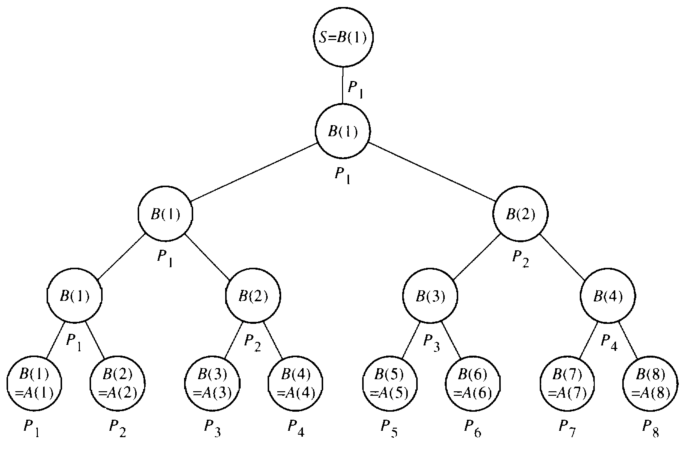
\includegraphics[width=34em]{images/pram_sum}
% \caption{Algorytm sumowania ośmiu elementów w modelu PRAM z osmioma procesorami. Każdy wewnętrzny wierzchołek grafu reprezentuje operację sumowania.}
% \label{fig:pram_sum}
% \end{figure}


\subsubsection{Algorytm mnożenia}
Rozważmy problem obliczenia iloczynu \(\mathbf{C}\) dwóch macierzy \(\mathbf{A}\), \(\mathbf{B}\in\mathbb{R}^{n\times n}\), gdzie \(n=2^k\), dla pewnego \(k\in\mathbf{N}\). Załóżmy, że dysponujemy \(n^3\) procesorami \(P_{i,j,l}\), \(1\leq i, j, l \leq n\) maszyny PRAM. Wówczas dla każdej pary \((i, j)\), n procesorów \(P_{i,j,l}\), gdzie \(1\leq l \leq n\), oblicza sumę \(\sum_{l=1}^{n}A(i,l)B(l,j)\) w myśl algorytmu \ref{alg:pram_sum}.\\

\alglanguage{pseudocode}
\begin{algorithm}
\centering
\begin{algorithmic}
\ParFor{\(P_{i,j,k}, \: 1 \leq i, \, j, \, k \leq n\)}
\State \(t[i,j,k] := a[i,k]*b[k,j]\)\Comment{Obliczanie składowych iloczynów skalarnych}
\EndParFor
\For{\(l \gets 1, \log{n}\)} \Comment{Sumowanie składowych iloczynów skalarnych}
	\ParFor{\(P_{i,j,k}, \: 1 \leq i, \, j \leq n, \, 1 \leq k \leq n/2^l \)}
	\State \(t[i,j,k] := T[i,j,2*k-1]+t[i,j,2*k]\)
\EndParFor
\EndFor

\ParFor{\(P_{i,j,k}, \: 1 \leq i, \, j \leq n, \, k = 1 \)}
\State \(c[i,j] := t[i,j,1] \)
\EndParFor
\end{algorithmic}
\caption{Algorytm mnożenia macierzy w siatce trójwymiarowej}
\label{alg:pram_sum}
\end{algorithm}


% \label{alg:crew_pram_multiplication}
% \begin{algorithm}[H]
% \SetKwData{Left}{left}\SetKwData{This}{this}\SetKwData{Up}{up}
% \SetKwFunction{Union}{Union}\SetKwFunction{FindCompress}{FindCompress}
% \SetKwInOut{Input}{wejście}\SetKwInOut{Output}{wyjście}
% \Input{Macierze \(\mathbf{A}\), \(\mathbf{B}\in\mathbb{R}^{n\times n}\), gdzie \(n=2^k\), dla pewnego \(k\in\mathbf{N}\) przechowywanych we wspólnej pamięci. Lokalnie zainicjalizowane zmienne to \(n\) i trójka wskaźników \((i, j, l)\)}
% \Output{Iloczyn \(\mathbf{C=AB}\) w pamięci współdzielonej}
% \begin{enumerate}
%  \item \( \mathtt{Oblicz}\quad C'(i,j,l) = A(i,l)B(l,j) \)
%  \item for \(h = 1\) to \( \log{n}\) do\\
%  if \(l \leq n/2^k\) then \texttt{Ustaw} \(C'(i,j,l):=C'(i,j,2l-1)+C'(i,j,2l)\)
%  \item \(if(l=1)\) then \texttt{Ustaw} \(C(i,j):=C'(i,j,1)\)
% \end{enumerate}
% \caption{Algorytm mnożenia macierzy w modelu PRAM\label{alg:pram_pseudokod}}
% \end{algorithm}

\begin{uwaga}
Algorytm \ref{alg:crew_pram_multiplication} wymaga równoległego odczytu ponieważ w trakcie wykonania kroku (1) procesory \(P_{i,l,k}\) mogą równocześnie odczytywać te same dane. Przykładowo procesory \(P_{i,1,l},P_{i,2,l},\dots,P_{i,n,l}\) w trakcie wykonywania kroku (1) wszystkie wymagają dostępu do \(A(i,l)\).
\end{uwaga}

% \subsection{Blokowa procedura \texttt{gaxpy}}
% Załóżmy, że \(A, B, C \in \mathbb{R}^{n\times n}\), gdzie \(B\) jest macierzą górnie trójkątną oraz obliczenie wielokrotnie nadpisuje dane
% \begin{align}
% D=C+AB
% \end{align}
% na komputerze z pamięcią współdzieloną przez \(p\) węzły. Załóżmy ponadto, że \(n=rkp\)

% \begin{align}
% [D_1, D_2, \dots, D_{kp}] = [C_1, C_2, \dots, C_{k*p}] + [A_1, A_2, \dots, A_{kp}] [B_1, B_2, \dots, B_{kp}]
% \end{align}
% gdzie każdy blok ma szerekość \(r=n/(kp)\). Jeśli
% \begin{align*}
% B_j=
% \begin{pmatrix}
% B_{1j}\\
% \vdots\\
% B_{jj}\\
% 0\\
% \vdots\\
% 0\\
% \end{pmatrix},
% \quad
% B_{ij}\in\mathbb{R}^{r*r}
% \end{align*}
% wówczas
% \begin{align}
% D_j = C_j + AB_j = C_j + \sum_{r=1}^{j}A_r B_{rj}.
% \end{align}

